\documentclass[tikz,border=10pt]{standalone}
\usetikzlibrary{calc}
\begin{document}
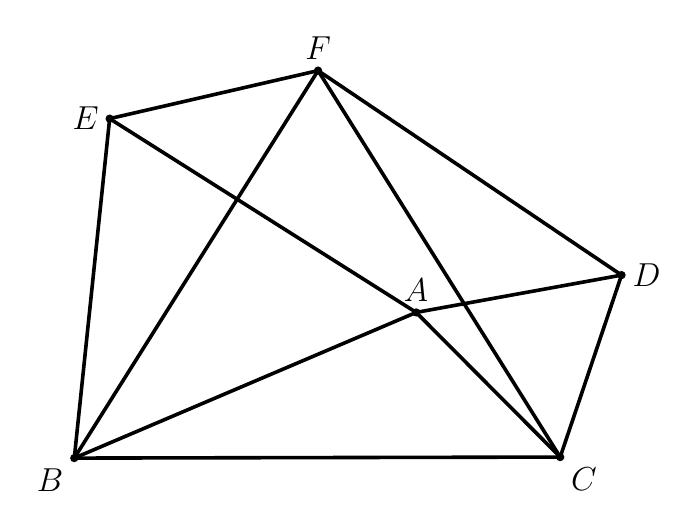
\begin{tikzpicture}[line width=1.3pt, line join=round]
\coordinate (A) at (0.847,-0.776);
\coordinate (B) at (-3.495,-2.626);
\coordinate (C) at (2.676,-2.613);
\coordinate (D) at (3.455,-0.302);
\coordinate (F) at (-0.399,2.295);



\coordinate (E) at (-3.046,1.685);


\draw (E) -- (F) -- (D) -- (C) -- (B) -- (E);
\draw (B) -- (F);
\draw (F) -- (C);
\draw (E) -- (A) -- (C);
\draw (B) -- (A) -- (D);

\foreach \p in {A,B,C,D,E,F} \fill (\p) circle (1.500pt);


\node[left] at (E) {\fontsize{13}{15.6}\selectfont $E$};
\node[above] at (F) {\fontsize{13}{15.6}\selectfont $F$};
\node[right] at (D) {\fontsize{13}{15.6}\selectfont $D$};

\node[above] at (A) {\fontsize{13}{15.6}\selectfont $A$};
\node[below right] at (C) {\fontsize{13}{15.6}\selectfont $C$};
\node[below left] at (B) {\fontsize{13}{15.6}\selectfont $B$};
\end{tikzpicture}
\end{document}